\documentclass[a4paper,12pt]{article} 

%%% Работа с русским языком
\usepackage{cmap}                           % поиск в PDF
\usepackage{mathtext} 			 	       % русские буквы в формулах
\usepackage[T2A]{fontenc}               % кодировка
\usepackage[utf8]{inputenc}              % кодировка исходного текста
\usepackage[english,russian]{babel}  % локализация и переносы

%Матеша
\usepackage{amsmath,amsfonts,amssymb,amsthm,mathtools} % AMS
\usepackage{icomma} % "Умная" запятая

%\mathtoolsset{showonlyrefs=true} % Показывать номера только у тех формул, на которые есть \eqref{} в тексте.

%% Шрифты
\usepackage{euscript}	 % Шрифт Евклид
\usepackage{mathrsfs} % Красивый матшрифт

%% Свои команды
\DeclareMathOperator{\sgn}{\mathop{sgn}}

%% Перенос знаков в формулах (по Львовскому)
\newcommand*{\hm}[1]{#1\nobreak\discretionary{}
{\hbox{$\mathsurround=0pt #1$}}{}}

%%% Заголовок
\author{Злобина Вера Б02-002}
\title{Лабораторная работа 2.4.1

Определение теплоты испарения жидкости}
\date{\today}

\begin{document}
	
\maketitle 
	
	
\newpage


\subparagraph*{Цель работы:}1) измерение давления насыщенного пара жидкости при разной температуре; 2) вычисление по полученным данным теплоты испарения с помощью уравнения Клапейрона-Клаузиуса. 
	
\subparagraph*{В работе используются:}термостат; герметический сосуд, заполненный исследуемой жидкостью; отсчётный микроскоп. 



\begin{figure}[h]	\label{plan1}
	
	\center{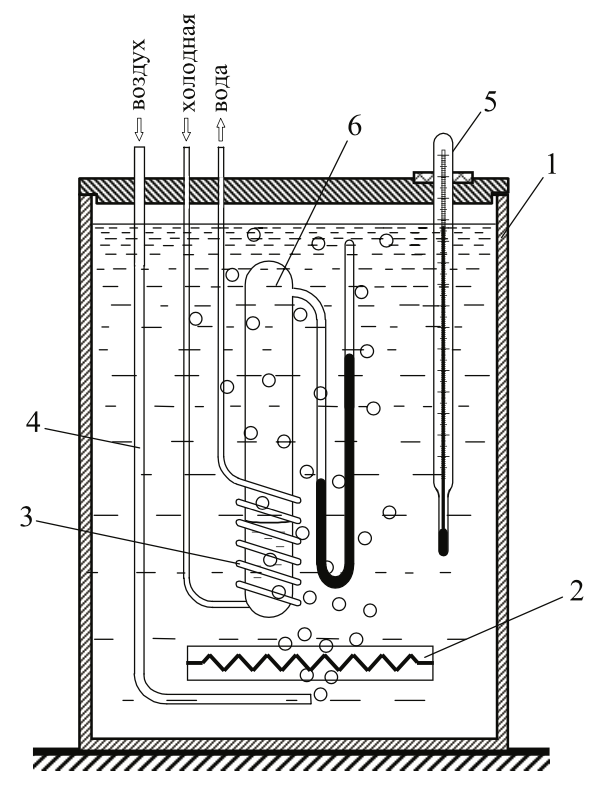
\includegraphics[width= 0.5\linewidth]{IMG_2.jpg}}
	\caption{Схема установки для определения теплоты испарения}

\end{figure}	

\begin{figure}[b!]	\label{plan2}
	
	\center{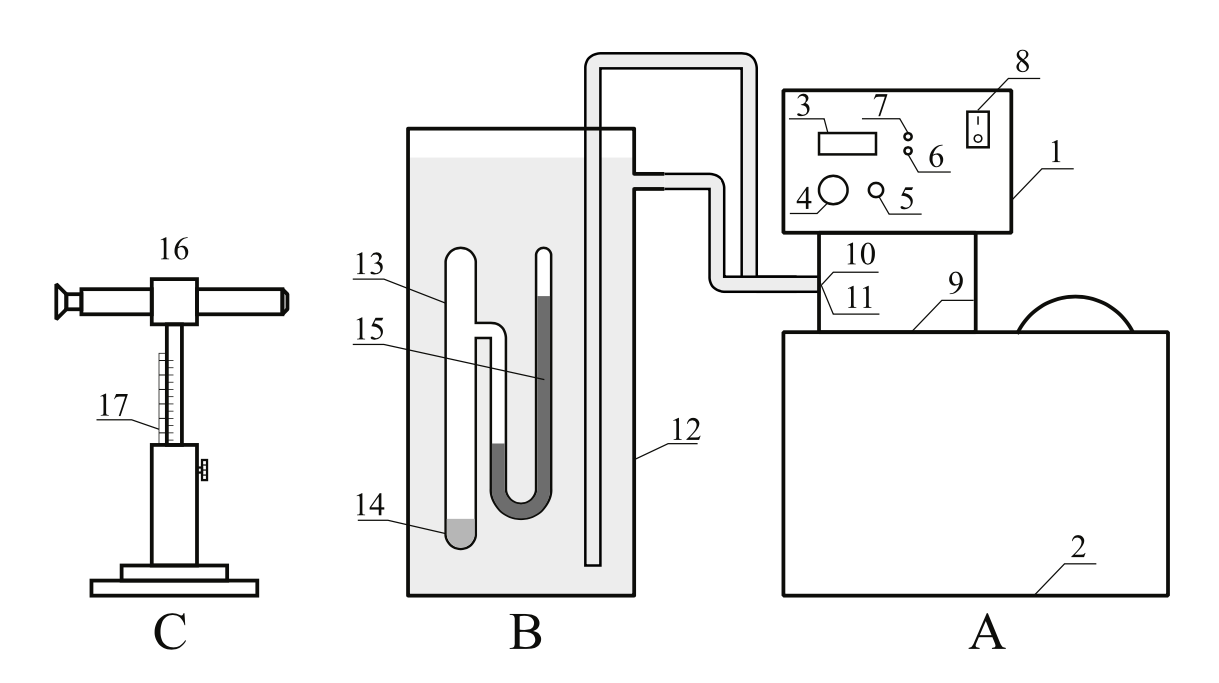
\includegraphics[width=1 \linewidth]{IMG_1.jpg}}
	\caption{Более полная схема установки}

\end{figure}




Испарением называется переход вещества из жидкого в газообразное состояние. Оно происходит на свободной поверхности жидкости. При испарении с поверхности вылетают молекулы, образую над ней пар. Для выхода из жидкости молекулы должны преодолеть силы молекулярного сцеления. Кроме того, при испарении совершается работа против внешнего давления $P$, поскольку объём жидкости меньше объёма пара. Не все молекулы жидкости способны совешить эту работу, а только те из них, кто обладает достаточной кинетической энергией. Поэтому переход части молекул в пар приводит к обеднению жидкости быстрыми молекулами, т. е. к её охлаждению. Чтобы испарение проходило без изменения температуры, к жидкости нужно подводить тепло. Количество теплоты, необходимое для изотермического испарения одного моля жидкости при внешнем давлении, равном упругости её насыщенных паров, называется её молярной теплотой испарения (парообразования). 

Теплоту парообразования жидкостей можно измерить непосредственно при помощи калориметра. Такой метод, однако, не позволяет получить точных результатов из-за неконтролируемых потерь тепла, которые трудно сделать малыми. В настоящей работе для определения теплоты испарения применен косвенный метор, основанный на формуле Клапейрона-Клаузиуса: 
\begin{equation} \label{kk}
 \dfrac{dP}{dT}= \dfrac{L}{T(V_2 - V_1)}. 
\end{equation}
Здесь  $P$ -- давление насыщенного пара жидкости при температуре  $T$,  $T$ -- абсолютная температура жидкости и пара, $L$ -- теплота испарения жидкости,  $V_1$ -- объём шара,  $V_2$ -- объём жидкости. Найдя из опыта  $dP/dT, T, V_2$ и $V_1$, можно определить $L$ путём рассчёта. Величины $L, V_2$ и $V_1$ в формуле \eqref{kk} должны относиться к одному и тому же количеству вещества; мы будем относить их к одному молю. 

В нашем приборе измерения проводятся при давлениях ниже атмосферного. В этом случае задача существенно упрощается. 

В таблице для ряда жидкостей приведены: температура, при которой давление насыщенных паров равно атмосферному, величины $V_1$ и $V_2$, входящие в \eqref{kk}, а так же константы $a$ и $b$ в уравнении Ван-дер-Ваальса. 


\begin{center}
\begin{tabular}{|l|*{6}{c|}} 
	\hline
	& $T_{кип}$,&$ V_1$, &$ V_2 , $&$ b$,& $ a$, & $a / V^2$, \\
	Вещество&  & $10^{-6}$ &$10^{-3}$&$10^{-6}$&& \\
	& К &$\frac{м^3}{моль} $&$\frac{м^3}{моль} $&$\frac{м^3}{моль} $&$\frac{Па \cdot м^6}{моль^2} $ &кПа\\ 
	\hline 
	Вода & 373 & 18 & 31 & 26 & 0,4& 0,42 \\ 
	CCl$_4$ & 350 & 97 & 29 & 126 & 1.95 & 2,3 \\ 
	Этиловый эфир & 307 & 104 & 25 & 137 & 1,8 & 2,9 \\ 
	Этиловый спирт & 351 & 58 & 29 & 84 & 1,2 & 1,4 \\ \hline
	\end{tabular}
\end{center}


Из таблицы видно, что $V_1$ не превосходит $0,5 \%$  от  $V_2$. При нашей точности опытов величиной $V_1$ в \eqref{kk} можно пренебречь. 

Обратимся теперь к $V_2$, которое в дальнейшем будем обозначать просто $V$. Объём $V$  связан с давлением и температурой уравнением Ван-дер-Ваальса:
\begin{equation} \label{vv}
\left(P + \dfrac{a}{V^2}\right)\left(V - b\right)= RT.
\end{equation}
Из таблицы можно видеть, что $b$ одного порядка с $V_1$. В уравнении Ван-дер-Ваальса величиной $b$ следует пренебречь. Пренебрежение членом $a/V^2$  по сравнению с $P$ вносит ошибку меньше $3\%$ . При давлении ниже атмосферного ошибки становятся ещё меньше. Таким образом, при давлениях ниже атмосферного уравнение Ван-дер-Ваальса для насыщенного пара мало отличается от уравнения Менделеева-Клапейрона. Положим поэтому
\begin{equation} \label{ig}
V = \frac{RT}{P}.
\end{equation}
Подставляя \eqref{ig} в \eqref{kk}, пренебрегая $V_1$ и разрешая уравнение относительно $L$, найдём 
\begin{equation} \label{res}
L = \frac{RT^2}{P}\frac{dP}{dT}=-R\frac{d(\ln P)}{d(1/T)}
\end{equation}
Эта формула является окончательной. 

В нашем опыте температура жидкости измеряется термометром, давление пара определяется  при помощи манометра, а производная $dP / dT$ $d(\ln P) / d(1 / T) $ находятся графически как угловой коэффициент касательной к кривой $P(T)$ или соответственно к кривой, у которой по оси абсцисс отложено $1/T$, а по оси ординат $\ln P$. 

\subparagraph*{Экспериментальная установка.} Cхема установки изображена на рис. 1 Наполненный водой резервуар 1 играет роль термостата. Нагревание термостата производится спиралью 2, подогреваемой электрическим током. Для охлаждения воды в термостате через змеевик3 пропускается водопроводная вода. Вода в термостате перемешивается воздухом, поступающим через трубку 4. Температура воды измеряется термометром 5. В термостат погружен запаянный прибор 6 с исследуемой жидкостью. Над ней находится насыщенный пар (перед заполнением прибора воздух из него был откачан). Давление насыщенного пара определяется по ртутному манометру, соединённому с исследуемым объёмом. Отсчёт показаний манометра производится при помощи микроскопа. 

Описание прибора указывает на второе важное преимущество предложенного косвенного метода измерения $L$ перед прямым. При непосредственном измерении теплоты испарения опыты нужно производить при неизменном давлении, и прибор может быть не запаян. При этом невозможно обеспечить такую чистоту и неизменность экспериментальных условий, как при нашей постановке опыта. 

Описываемый прибор обладает важным недостатком: термометр определяет температуру термостата, а не исследуемой жидкости (или её пара). Эти температуры близки друг к другу лишь в том случае, если нагревание происходит достаточно медленно. Убедиться в том, что темп нагревания не является слишком быстрым, можно, сравнивая результаты, полученные при нагревании и при остывании прибора. Такое сравнение необходимо сделать. Для ориентировки укажем, что температуру воды в калориметре следует менять не быстрее, чем на $1^{\circ}$С в течение 1---3 минут. 


\newpage

\section*{Ход работы}

\subparagraph*{1.} Измерим высоты, на которых расположены мениски в ртутном U-образном манометре с помощью микроскопа и температуру по  индикаторному табло. Вычислим разность уровней $\Delta h$. Данные занесём в Таблицу 1. 

\subparagraph*{2.} Продолжая повышать температуру нагреем жидокость до температуры $\approx 40^{\circ}$С,
через каждый градус будем проводить те же измерения, занося данные в Таблицу 1. 



\begin{table}[h!] 
	\caption{Экспериментальные данные}
	\begin{center}
	\begin{tabular}{|*{4}{l|}}
		\hline 
		$T$,&$h_1$,&$h_2$,&$\Delta h$,\\ 
		$^{\circ}$C&мм&мм&мм\\ \hline

		21,03 &79,9 &99,2 &19,3  \\ \hline 
		22,07&79,1&99,2&20,1  \\ \hline 
		23,09&78,3&99.8&21,5 \\ \hline 
		24,07&77,7&100,1&22,9 \\ \hline 
		25,03&77,1&100,3&24,5\\ \hline 
		26,08& 76,0&101,9&25,9 \\ \hline 
		27,06 &75,7 &103,0&27,3  \\ \hline 
		28,05 &74,5&104,0&29,5     \\ \hline 
		29,09 &73,9&104,4 &30,5      \\ \hline 
		30,09 &72,8&105,0&32,2      \\ \hline 
		31,07 &72,2&106,6&34,4      \\ \hline 
		32,05 &70,9&107,6&36,7     \\ \hline 
		33,04&70,0 &107,9&37,9      \\ \hline 
		34,07&69,2&109,4&40,2      \\ \hline 
		35,05 &68,3&110,1&41,8     \\ \hline 
		36,04 &67,0&110,8&43,8      \\ \hline 
		37,03 &65,9&111,7&45,8      \\ \hline 
		38,03 &64,9&113,5    &48,6     \\ \hline 

	\end{tabular}

\end{center}
\end{table}



\subparagraph*{3.}  По разности уровней жидкости рассчитаем давление, используя формулу $P = \rho_{рт} g \Delta h$. По полученным данным построим графики в координатах $T$,  $P$ (рис. 3)  и в координатах $1/T$,  $\ln P$ (рис. 4). 

По формуле \eqref{res} вычислим $L$.


\subparagraph*{1 способ:} для реализации этого способа нужно найти производную функции $P(T)$ в каждой из имеющихся на первом графике (рис. 3) точек. Мы сделаем это таким методом: каждую тройку ближайших точек аппроксимируем параболой и запишем значения коэффициента, отвечающего за угол наклона касательной к параболе в центральной точке. Полученные значения запишем в Таблицу 2.

 


\begin{table}[h!] 
	\caption{Вычисление коэффициента $L$}
	\begin{center}
		\begin{tabular}{|*{9}{l|}}
			\hline 
		
			
			
				$T$,$^{\circ}$C & 22,07&	23,09&	24,07&	25,03&26,08& 27,06 &28,05 &29,09 \\ \hline
				$L$б кДж/кг& 2234 & 2397 & 2519 & 2283& 2327 & 2256& 2493& 2537 \\ \hline
				$T$,$^{\circ}$C  &	30,09 &	31,07 &	32,05 &	33,04&	34,07&35,05 &36,04 &	37,03  \\ \hline
				$L$, кДж/кг& 2544&2438& 2371&2695&2739&2674& 2715&2856 \\ \hline
		\end{tabular}
		
	\end{center}
\end{table}

Тогда статистическая погрешность искомой велилчины $  \sigma _{ст}L\approx 0,3 МДж/кг$, то есть $\varepsilon_{ст} \approx 13\%$ , в то время как приборная погрешность $\varepsilon_{пр}\approx \frac{2\sigma\Delta h}{\Delta h} =1,5\% $, а значит ей можно принебречь в сравнении с погрешностью предложенного метода. Тогда итоговый результат: 

$$L = (2,5 \pm 0,3) МДж  / кг$$


\begin{figure}[h!]	
	
	\center{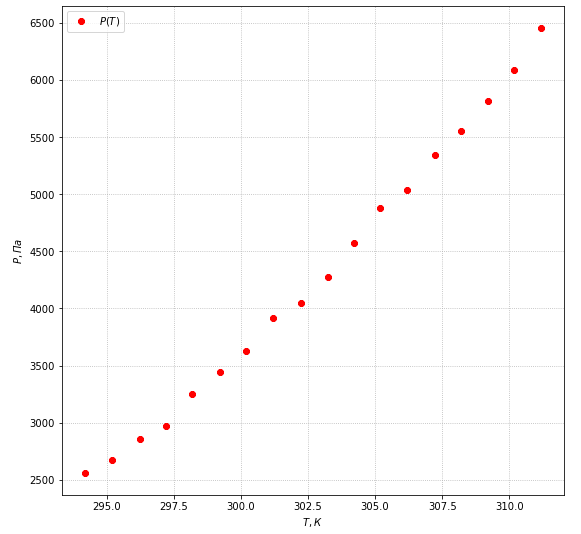
\includegraphics[width= 0.6\linewidth]{5.jpg}}
\caption{График зависимости $P(T)$}
	
\end{figure}	

\newpage
\subparagraph*{2 способ:} теперь воспользуемся вторым графиком (рис. 4). Здесь величина $L$ это просто коэффициент наклона прямой, значение которого мы получаем с помощью МНК. 


Здесь же болший вклад в погрешность вносит инструментальная погрешность, поэтому итоговое значение $L$, полученное этим способом 


При этом табличное значение искомой величины L = 2,26 МДж/кг. 

$$
L =( 2,29 \pm 0,05) МДж/кг 
$$


\begin{figure}[h!]	\label{plan1}
	
	\center{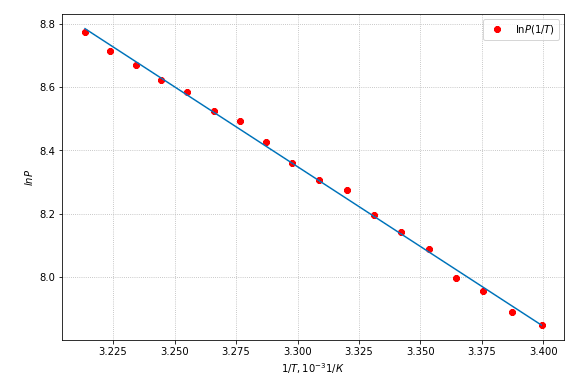
\includegraphics[width= \linewidth]{6.jpg}}
	\caption{График зависимости $\ln P (1/T)$}
	
\end{figure}




	
\newpage

\section*{Вывод}


В результате эксперимента у нас получилось двумя способами рассчитать значение удельной теплоты парообразования для воды, которые совпали с табличным значением. Стоит отметить, что первый способ дал погрешность, почти на порядок большую, чем второй. Этот метод плох тем, что нужно было по точкам вычислять производную, а этого не получилось сделать с приемлимой точностью. Обусловлено это тем, что даже одна точка, учитывается при вычислениях три раза, поэтому вносит большую погрешность. Более точным оказался второй метод, где теоретически было обусловлено, что полученные точки должны лежать на одной прямой, исходя из чего легко находился нужный коэффициент. Из двух полученных графиков информативным можно назвать только второй. 

Факт того, что мы получили значение удельной теплоты парообразования, совпадающее с табличным, говорит нам о том, что мы правильно восполльзовались приближением водяного пара как идеального газа. 



\end{document}



